
\documentclass[12pt]{article}
\usepackage{amsmath}
\DeclareMathOperator*{\argmin}{arg\,min} % thin space, limits underneath in displays
\DeclareMathOperator*{\argmax}{arg\,max} % thin space, limits underneath in displays
\newtheorem{thm}{Theorem}
\usepackage{amssymb}
\usepackage{amsfonts}
\usepackage{mathrsfs}
\usepackage{bm}
\usepackage{indentfirst}
\setlength{\parindent}{0em}
\usepackage[margin=1in]{geometry}
\usepackage{graphicx}
\usepackage{setspace}
\doublespacing
\usepackage[flushleft]{threeparttable}
\usepackage{booktabs,caption}
\usepackage{float}
\usepackage{graphicx}
\usepackage[sort,comma]{natbib}
\usepackage[hidelinks]{hyperref}

\usepackage{import}
\usepackage{xifthen}
\usepackage{pdfpages}
\usepackage{transparent}

\newcommand{\incfig}[1]{%
\def\svgwidth{\columnwidth}
\import{./figures/}{#1.pdf_tex}
}




\title{The Solow Growth model}
\author{}
\date{}


\begin{document}
\maketitle

{\textbf {Conclusion:}}

the accumulation of physical capital cannot account for (explain) either the vast 
growth over time in output per person, $ g_{\frac{Y}{L}} $, or the vast geographic 
differences in output per person.

The model treats other potential sources of differences in real incomes, $ Y $, as
either exogenous (e.g., technological progress) or absent altogether (e.g., positive 
externalities from capital).

It does not investigate the determinants of saving and investment.



\section{Assumptions}



\subsection{Four variables: }
\begin{itemize}
\item output, $ Y $
\item capital, $ K $
\item labor, $ L $
\item knowledge, or the effectiveness of labor, $ A $
\end{itemize}


Ignore other inputs, e.g., natural resources.



\subsection{Production function:}

\subsubsection{Labor-augmenting}
\begin{equation*}
Y(t) = F[K(t), A(t)L(t)]
\end{equation*}

It says technology progress is labor-augmenting or Harrod-neutral.

================================\\
Note:\\
Technology progress is capital-augmenting if $ Y = F(AK,L) $\\
Technology progress is Hicks-neutral if $ Y = AF(K,L) $\\
================================


\subsubsection{CTRS}
Production function is constant return to scale in $ K $ and $ AL $. 
\begin{equation*}
F(\lambda K, \lambda AL) = \lambda F(K, AL),\quad \forall \lambda \ge 0.
\end{equation*}

If we let $ \lambda = \frac{1}{AL} $,
\begin{align*}
F \left( \frac{K}{AL},1 \right)  &= \frac{1}{AL}F(K,AL)\\
\frac{K}{AL}&: \text{ capital per effective labor }\\
\frac{1}{AL}F(\cdot ) = \frac{Y}{AL}&: \text{ output per effective labor }
\end{align*}

Define:
\begin{align*}
k &= \frac{K}{AL}\\
y &= \frac{Y}{AL}\\
y &= f(k) = F(k,1) = F \left( \frac{K}{AL},1 \right) = \frac{1}{AL}F(K,AL)\\
\frac{Y}{L}&= A \left( \frac{Y}{AL} \right)  = Af(k)
\end{align*}

\subsubsection{Quasi-concave}
For $ f(k) $,
\begin{equation*}
f(0) = 0, \quad f'(k) > 0, \quad f''(k) < 0
\end{equation*}

Since 
\begin{equation*}
F(K,AL) = AL f(K/AL),
\end{equation*}
the MPK would be
\begin{align*}
MPK &= AL f'\left( \frac{K}{AL} \right) \frac{1}{AL} = f' (k) > 0.
\end{align*}

And
\begin{align*}
\lim_{k \to \infty} f'(k) &= 0\\
\lim_{k \to 0} f'(k) &= \infty 
\end{align*}


Consider a Cobb-Douglas production function
\begin{equation*}
F(K,AL) = K^{\alpha}(AL)^{1 - \alpha}, \quad \alpha \in (0,1)
\end{equation*}
\begin{align*}
f(k)&= F \left( \frac{K}{AL}, 1 \right) \\
&= \left( \frac{K}{AL} \right) ^{\alpha}\\
&= k ^{\alpha}\\
f'(k)&= \alpha k ^{\alpha - 1}
\end{align*}




\subsection{Accumulation of inputs}
$ K_0, L_0, A_0 $ are given and strictly positive.

Growth rate of $ L $ and $ A $
\begin{align*}
\dot{L}(t)&= nL(t)\\
\dot{A}(t)&= gA(t),
\end{align*}
where $ n,g $ are exogenous.

{\textbf {Capital accumulation}}
\begin{equation*}
		\dot{K}(t)  = [Y(t) - C(t)] - \delta K(t) = I(t) - \delta K(t)
\end{equation*}

\noindent\fbox{%
\parbox{\textwidth}{%
The only substantial differences among Solow, Ramsey, and Diamond overlapping-
generations model concern their assumptions about how output is divided between
Consumption and Investment.

In both Ramsey and Diamond models, divisions arises endogenously.
}%
}\\


In the Solow model, the division is taken as given, the exogenous saving rate ($ s $).
\begin{equation*}
\dot{K}(t) = sY(t) - \delta K(t), \quad s \in (0,1]
\end{equation*}




Recall, $ k(t) = K(t)[A(t)L(t)]^{ - 1} = \frac{K(t)}{A(t)L(t)} $, then
\begin{align*}
\frac{dk(t)}{dt} = \dot{k}(t)
&= \dot{K}(t)[A(t)L(t)]^{ - 1} - K(t)[A(t)L(t)]^{ - 2}[\dot{A}(t)L(t) + A(t)\dot{L}(t)]
\\
&= \frac{\dot{K}}{AL} - \frac{K}{(AL)^{2}}\dot{A}L - \frac{K}{(AL)^{2}}A\dot{L}\\
&= \frac{\dot{K}}{AL} - \frac{K}{AL}\frac{\dot{A}L}{AL} - \frac{K}{AL}\frac{A\dot{L}}{
AL}\\
&= \frac{\dot{K}}{AL} - \frac{K}{AL}\frac{\dot{A}}{A} - \frac{K}{AL}\frac{\dot{L}}{L}\\
&= \frac{sY - \delta K}{AL} - kg - kn, \quad 
\text{ since $ \dot{K} =  sY - \delta K$ }\\
&= \frac{sY}{AL} - k \delta - kg - kn\\
\dot{k}&= sf(k) - (\delta + g + n)k
\end{align*}
This is the key equation of the Solow model.

\begin{figure}[H]
\center{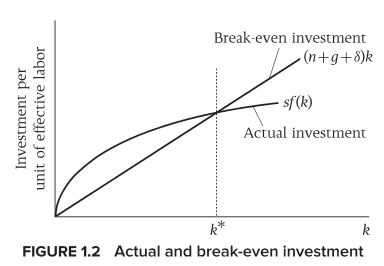
\includegraphics[scale =.8 ]  {figures/solow_investment_actual-break-even.png}}
\end{figure}

If $ k < k ^{*} $ , actual investment is greater than the break-even investment, so
$ k $ is rising.

$ k $ converges to $ k ^{*} $.


\subsection{Balanced growth path}

\begin{equation*}
k = \frac{K}{AL} \rightarrow K = ALk, \quad g_{K} = g_{A} + g_{L} + 0 = g + n
\end{equation*}

When $ k = k ^{*} $, $ k $ is constant,

$ K $ grows at rate $ g + n $,

$ \frac{Y}{L} $ grows at rate $ g $

The Solow model implies that {\textbf {regardless of its starting point, the economy
converges to a balance path--a situation where each variable is growing at a constant
rate. The growth rate of output per worker, $ \frac{Y}{L} $, is determined solely
by the rate of technological progress, $ g $.}}


\subsection{The impact of a change in the saving rate}

\begin{figure}[H]
\center{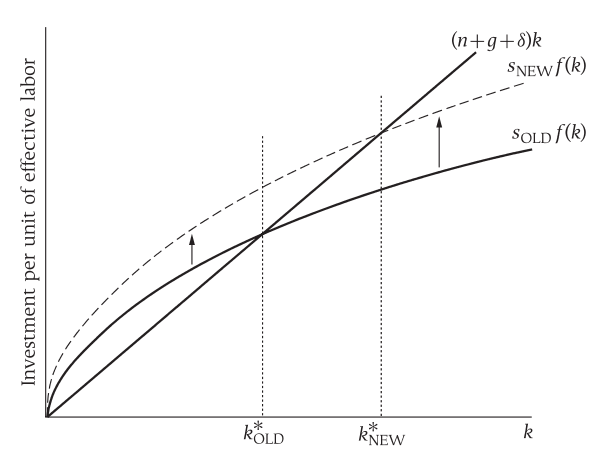
\includegraphics[scale =.5 ]  {figures/change_in_saving.png}}
\end{figure}

\begin{figure}[H]
\center{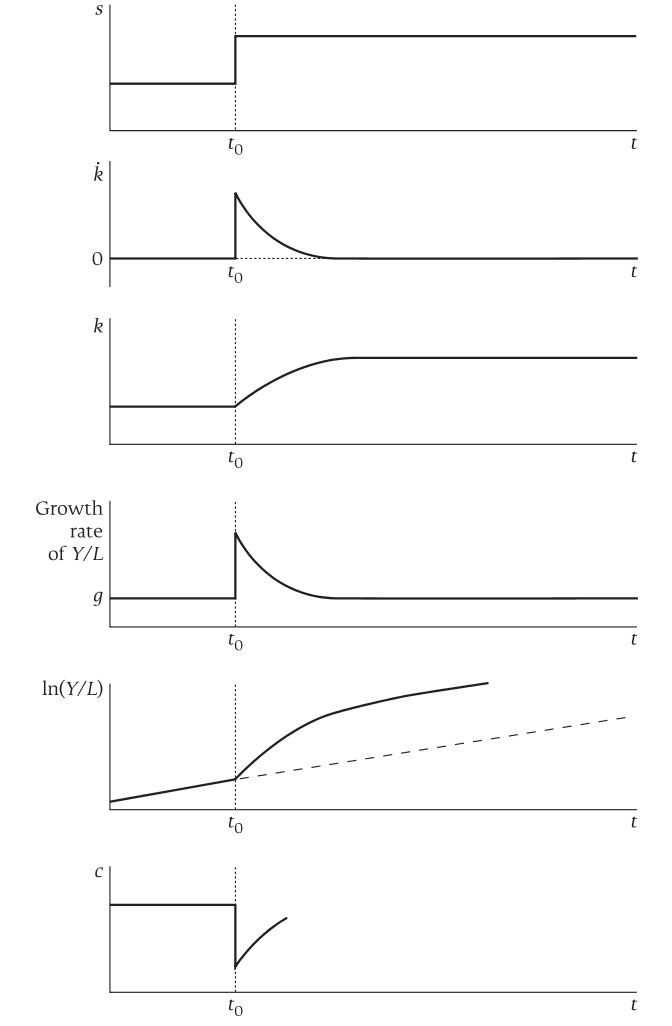
\includegraphics[scale =.5 ]  {figures/solow_impact_saving.png}}
\end{figure}

The growth rate of $ \frac{Y}{L} $:
recall $ \frac{Y}{L} = Af(k) $, a permanent increase in $ s $ causes $ k $ to increase,
hence, $ \frac{Y}{L} $ grows both because $ A $ and $ k $. It follows the path
of $ \dot{k} $ because when $ k $ approach to new SS, $ \dot{k} = 0 $, so $ \frac{Y}{L}
$ goes back to previous growth rate, $ g $.

Hence, change in the saving rate has a {\textbf {level effect}}, but not a 
{\textbf {growth effect}}.


\subsection{The impact on Consumption}


























\end{document}

